%% LyX 2.0.2 created this file.  For more info, see http://www.lyx.org/.
%% Do not edit unless you really know what you are doing.
\documentclass[twocolumn,english]{IEEEtran}
\usepackage[T1]{fontenc}
\usepackage{babel}
\usepackage{amsthm}
\usepackage{graphicx}
\usepackage[unicode=true,
 bookmarks=true,bookmarksnumbered=true,bookmarksopen=true,bookmarksopenlevel=1,
 breaklinks=false,pdfborder={0 0 0},backref=false,colorlinks=false]
 {hyperref}
\hypersetup{pdftitle={Your Title},
 pdfauthor={Your Name},
 pdfpagelayout=OneColumn, pdfnewwindow=true, pdfstartview=XYZ, plainpages=false}

\makeatletter

%%%%%%%%%%%%%%%%%%%%%%%%%%%%%% LyX specific LaTeX commands.
\DeclareRobustCommand*{\lyxarrow}{%
\@ifstar
{\leavevmode\,$\triangleleft$\,\allowbreak}
{\leavevmode\,$\triangleright$\,\allowbreak}}
%% Because html converters don't know tabularnewline
\providecommand{\tabularnewline}{\\}

%%%%%%%%%%%%%%%%%%%%%%%%%%%%%% Textclass specific LaTeX commands.
 % protect \markboth against an old bug reintroduced in babel >= 3.8g
 \let\oldforeign@language\foreign@language
 \DeclareRobustCommand{\foreign@language}[1]{%
   \lowercase{\oldforeign@language{#1}}}
\theoremstyle{plain}
\newtheorem{thm}{\protect\theoremname}
\theoremstyle{plain}
\newtheorem{lem}[thm]{\protect\lemmaname}

%%%%%%%%%%%%%%%%%%%%%%%%%%%%%% User specified LaTeX commands.
% for subfigures/subtables
\ifCLASSOPTIONcompsoc
\usepackage[caption=false,font=normalsize,labelfont=sf,textfont=sf]{subfig}
\else
\usepackage[caption=false,font=footnotesize]{subfig}
\fi

\makeatother

\providecommand{\lemmaname}{Lemma}
\providecommand{\theoremname}{Theorem}

\begin{document}





\title{Peak2Cloud: Scientific Computing in the Cloud}


\author{Joseph Anthony C.~Hermocilla %
\thanks{e-mail: \protect\href{mailto:jchermocilla@up.edu.ph}{jchermocilla@up.edu.ph}.%
}}


\markboth{ICS Technical Reports, Vol. 2014, No. 1, January-June 2014}{Joseph
Anthony Hermocilla : Peak2Cloud: Scientific Computing in the Cloud}


\IEEEpubid{\copyright~2014 Institute of Computer Science, University of the
Philippines Los Banos}
\maketitle
\begin{abstract}
Peak2Cloud (P2C) is an Openstack-based private cloud deployed as testbed
for scientific computing. We present how P2C was setup, configured,
and tested. We also describe vcluster, a tool for rapidly deploying
message-passing clusters on P2C. Finally, we show and analyze some
benchmark results on the message-passing performance of virtual clusters
deployed on P2C.\end{abstract}
\begin{IEEEkeywords}
cloud computing, scientific computing, message passing
\end{IEEEkeywords}

\section{Introduction}

\IEEEPARstart{ C}{loud} computing is becoming a popular choice
for deploying online services. \cite{iosup_performance_2011}


\section{Previous Work}

text text text text text text text text text text text text text text
text\cite{bourguiba_improving_2014}


\subsection{subsection}


\subsection{another subsection}


\section{Methodology}
\begin{thm}[Theorem name]
For a named theorem or theorem-like environment you need to insert
the name through \textsf{Insert\lyxarrow{}Short Title}, as done here.\end{thm}
\begin{lem}
If you don't want a theorem or lemma name don't add one.\end{lem}
\begin{IEEEproof}
And here's the proof!
\end{IEEEproof}

\section{Results}

\begin{figure}[htbp]
\begin{centering}
\textsf{A single column figure goes here}
\par\end{centering}

\caption{Captions go \emph{under} the figure}
\end{figure}
\begin{table}[htbp]
\caption{Table captions go \emph{above} the table}


\centering{}%
\begin{tabular}{|c|c|}
\hline 
delete & this\tabularnewline
\hline 
\hline 
example & table\tabularnewline
\hline 
\end{tabular}
\end{table}



\section{Conclusions}

bla bla


\appendices{}


\section{First appendix}

Citation: 


\section{Second appendix}


\section*{Acknowlegment}

Many thanks to the reviewers as well as to ICS.

\bibliographystyle{./IEEEtran}
\bibliography{p2cpaper}

\begin{IEEEbiography}[{{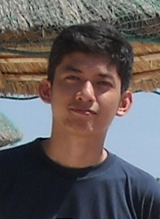
\includegraphics[clip,width=1in,height=1.25in]{me-new}}}]
{Joseph Anthony C. Hermocilla} obtained his MS in Computer Science
from the University of the Philippines Los Banos where he is currently
an assistant professor at the Institute of Computer Science and head
of the Systems Research Group. His research interests span the area
of systems, including operating systems, computer architecture, data
communications and networking, distributed systems, computer security,
and high-performance computing. He is a member of the Computing Society
of the Philippines and the Philippine Society of Information Technology
Educators.
\end{IEEEbiography}

\end{document}
